	\axioma{P1} Si tenemos el conjunto $\P$, denominado \textbf{plano}, y la aplicación $d:\P \times \P \rightarrow \R$ llamada \textbf{distancia}, entonces$(\P, d)$ es un espacio métrico.

\defi{2.2} Una \textbf{recta} $r \subset \P$ satisface
\begin{itemizex}
	\item $r$ contiene al menos dos puntos.
	\item Para toda terna de puntos $A, B, C$, están alineados si están en $r$.
\end{itemizex}

\axioma{P2} $\P$ contiene al menos tres puntos no alineados; y por dos puntos distintos, $A$ y $B$ de $\P$ pasa una recta, $r_{AB}$.

\defi{2.6} / \tma{2.7} Dos rectas se cortan si sólo tienen un punto en común, y si no tienen ningún punto en común, entonces se denominan \textbf{paralelas}, y se denota por $a \parallel b$. Dos rectas, o se cortan o son paralelas.

\importante\axioma{P3} Para toda recta $r \subset \P$ existe una biyección $\gamma: r \rightarrow \R$ tal que $|\gamma(X) - \gamma(Y)| = |x - y| = d(X, Y) \;\; \forall \;\; X,Y \in r$ 

\obs{2.8} Si $A, B \in r$ son distintos, entonces existe un punto $M\in r: d(A,M) = d(M,B)$ que denotamos por $\m[A,B]$ y se llama \textbf{punto medio}. Asimismo sólo existe un punto $B \in r$ tal que $B = \m[A, M]$.

\obs{2.9} Si $r$ es una recta y $P \in r$, entonces $r$ se puede dividir en dos \textbf{semirrectas}, que son los conjuntos $\{X \in r \; | \; \gamma(X) > \gamma(P)\}$ y $\{X \in r \; | \; \gamma(X) < \gamma(P)\}$.

\axioma{P4} Para toda recta $r \subset \P$ hay dos subconjuntos $H^1$ y $H^2$, denominados \textbf{semiplanos} de $r$, que verifican:
\begin{itemizex}
	\item $H^1 \cup H^2 = \P-r$
	\item Si $X,Y \in H^i$ entonces $[X,Y] \subset H^i$
	\item Si $X \in H^1$ y $Y \in H^2$ entonces $[X,Y] \cap r \neq \emptyset$.
\end{itemizex}

\defi{2.15} Sean $P, Q, R$ no alineados, entonces el triángulo $\triangle\{P,Q,R\}$, o $\triangle PQR$ está formado por los segmentos $[P,Q]$, $[Q,R]$, $[P,R]$, llamados lados, y los vértices $P,Q, R$.

\tma{2.16 [Axioma de Pasch]a} Dado un triángulo $\triangle PQR$ y una recta $r$; si $r$ corta a $[P,Q]$, entonces o corta a $[P,R]$ o a $[Q, R]$.

\defi{2.17 = 1.5} Una \textbf{isometría} en $\P$ es una biyección $g: \P \rightarrow \P$ que cumple que $d(g(X), g(Y)) = d(X,Y) \;\;\forall\;\; X,Y \in \P$.

\tma{2.18} Si $A,B \in \P$ y $g \in \iso(\P)$ entonces $g([A,B]) = [g(A), g(B)]$ y $g(r_{AB}) = r_{g(A)g(B)}$ 

\axioma{P5} Si $A_1, A_2 \in \P$ y $B_1, B_2 \in \P$ son dos pares de puntos que cumplen $d(A_1,A_2) = d(B_1,B_2)$ entonces existe $g \in \iso(\P)$ tal que $g(A_i) = B_i$. Se dice que esos pares de puntos son \textbf{congruentes}.

\axioma{P6} Para toda recta $r$ existe una isometría $\sigma$ llamada \textbf{reflexión} tal que  
\begin{itemizex}
	\item $\sigma(X) = X\iff X \in r$
	\item $\sigma \circ \sigma = \text{Id}$
\end{itemizex}


\defi{2.23} / \tma{2.25} / \cor{2.30} Una recta $l$ es \textbf{ortogonal} a $r$ si para todo $S \in l$ y para todo par de puntos $A, B$ que cumple que $M = \m[A,B]$, de modo que $l \cap r = M$, entonces se da que $d(A,S) = d(S,B)$. Se denota $l \perp_M r$. En estas condiciones, $l = \{X \in \P \; | \; d(S,A) = d(S,B)\}$, se denomina \textbf{mediatriz} de $[A,B]$. 

\begin{figure}[H]
	\centering
	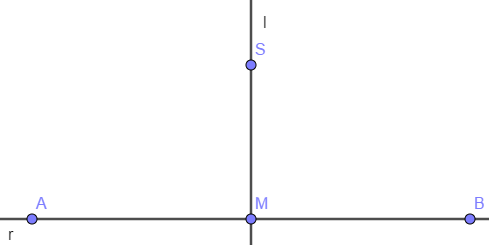
\includegraphics[width=7cm]{figuras/2-23.png}
	\vspace{-1em}
\end{figure}

\lema{2.21} Si $\sigma_r$ entonces, para todo $X$, $\m[X, \sigma_r(X)] \in r$.

\obs{2.24} Si $l \perp r$ y $g \in \iso(\P)$ entonces $g(l) \perp g(r)$.

\tma{2.26} Si $l, r \subset \P$ cortan en $M$ y $\sigma_l, \sigma_r$ son dos reflexiones de $l$ y $r$, entonces se cumple que $l \perp_M r \iff r \perp_M l \iff \sigma_r(l) = l \iff \sigma_l(r) = r$.

\tma{2.27 / 2.29} Para toda recta $r$ y todo punto $S \in \P - r$, existe una recta $l$ ortogonal a $r$, que pasa por $S$. Si $r$ es una recta, y $M \in r$, entonces existe $l$ tal que $l \perp_M r$.

\axioma{P7} Para toda recta $r$ y todo punto $P$ existe sólo una recta \textbf{paralela} a $r$ que pase por $P$.

\tma{2.31 / 2.33} Si $a \perp l$ y $b \perp l$ entonces $a \parallel b$. Sean $a \parallel b$. Entonces, para todo $A \in a$, la única recta $l \perp_A a$ también es ortogonal a $b$.

\tma{2.32} Las rectas parallelas forman una relación de recurrencia.
\begin{itemizex}
	\item Reflexividad: $a\parallel a$
	\item Simetría: $a \parallel b \rightarrow b \parallel a$
	\item Transitividad  $a \parallel b $ y  $b \parallel c \rightarrow a \parallel c$
\end{itemizex}

\ej{2.6} Sean $A,B \in r$, $A \neq B$. Para todo $t$, existe un único $P_t\in r$ que cumple $d(P_t,A) = \abs{t}$ y $d(P_t, B) = \abs{t-d(A,B)}$. En definitiva, la posición de $P_t$ está sólamente determinada por las distancias $d(A, P_t)$ y $d(P_t, B)$.
	 
	 
	 
	 
	 
	 
	 